
%%%
% Regularization to prevent too strong of weights
%%%

\subsubsection{Regularization}

%%%
% Process
%%%

%%%
As an attempt to prevent a single strategy's weight from being so strongly 
preferred that a second strategy could not hope to possibly gain ground,
a hard limit was placed on the pre-normalized update value.
%
Expressed mathematically,
\[
    w'_{m,o,d}[i] = \max\{K,cw_{m,o,d}[i]\}
\]
where $K$ is some constant value throughout the training.
%
While the value of $w_{m,o,d}[i]$ could exceed $K$ after re-normalization
for a particularly strongly weighted strategy,
the value could be seen converging to $K$ within a handful of iterations.
%
The desired intention of this regularization was to allow other strategies
the opportunity to overcome the bias of earlier strengthening of the strongest
strategy.
%%%

\paragraph{Results}

%%%
% Results:
%	Similar areas taken up for hand_max_{min,avg}
%		both share same space rather than Croatia/Boz&Herz-shape
%	Grayer, since values only so large
%	As max value is increased,
%		darker, more like un-regulated
%	Islands still present
%	losing, still uncertain
%		still chance of higher than regulation, because of aforementioned reason
%%%


\begin{figure}
\center

	\begin{subfigure}[t]{0.22\textwidth}
		\center
		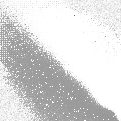
\includegraphics[width=\textwidth]{images/findings/experiments/regularization/strats/0.50/hand_max_min.png}
		\caption{\handmaxmin}
	\end{subfigure}
	~
	\begin{subfigure}[t]{0.22\textwidth}
		\center
		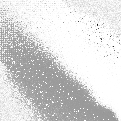
\includegraphics[width=\textwidth]{images/findings/experiments/regularization/strats/0.50/hand_max_avg.png}
		\caption{\handmaxavg}
	\end{subfigure}
~
	\begin{subfigure}[t]{0.22\textwidth}
		\center
		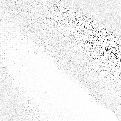
\includegraphics[width=\textwidth]{images/findings/experiments/regularization/strats/0.50/hand_max_med.png}
		\caption{\handmaxmed}
	\end{subfigure}
	~
	\begin{subfigure}[t]{0.22\textwidth}
		\center
		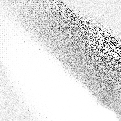
\includegraphics[width=\textwidth]{images/findings/experiments/regularization/strats/0.50/hand_max_poss.png}
		\caption{\handmaxposs}
	\end{subfigure}

	\begin{subfigure}[t]{0.22\textwidth}
		\center
		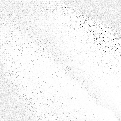
\includegraphics[width=\textwidth]{images/findings/experiments/regularization/strats/0.50/crib_min_avg.png}
		\caption{\cribminavg}
	\end{subfigure}
	~
	\begin{subfigure}[t]{0.22\textwidth}
		\center
		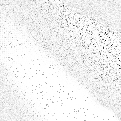
\includegraphics[width=\textwidth]{images/findings/experiments/regularization/strats/0.50/pegging_max_avg_gained.png}
		\caption{\peggingmaxavggained}
	\end{subfigure}
~
	\begin{subfigure}[t]{0.22\textwidth}
		\center
		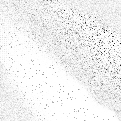
\includegraphics[width=\textwidth]{images/findings/experiments/regularization/strats/0.50/pegging_max_med_gained.png}
		\caption{\peggingmaxmedgained}
	\end{subfigure}
	~
	\begin{subfigure}[t]{0.22\textwidth}
		\center
		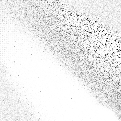
\includegraphics[width=\textwidth]{images/findings/experiments/regularization/strats/0.50/pegging_min_avg_given.png}
		\caption{\peggingminavggiven}
	\end{subfigure}

\caption{
	Final strategies for an agent using regularized learning
	when playing as the pone
	and the maximum value weight allowed is 0.50
	after training for 500,000 games.
}
\label{fig:reg-strats-0.50}
\end{figure}


\begin{figure}
\center

	\begin{subfigure}[t]{0.22\textwidth}
		\center
		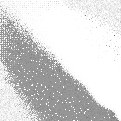
\includegraphics[width=\textwidth]{images/findings/experiments/regularization/strats/0.60/hand_max_min.png}
		\caption{\handmaxmin}
	\end{subfigure}
	~
	\begin{subfigure}[t]{0.22\textwidth}
		\center
		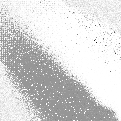
\includegraphics[width=\textwidth]{images/findings/experiments/regularization/strats/0.60/hand_max_avg.png}
		\caption{\handmaxavg}
	\end{subfigure}
~
	\begin{subfigure}[t]{0.22\textwidth}
		\center
		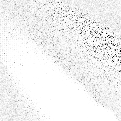
\includegraphics[width=\textwidth]{images/findings/experiments/regularization/strats/0.60/hand_max_med.png}
		\caption{\handmaxmed}
	\end{subfigure}
	~
	\begin{subfigure}[t]{0.22\textwidth}
		\center
		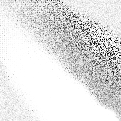
\includegraphics[width=\textwidth]{images/findings/experiments/regularization/strats/0.60/hand_max_poss.png}
		\caption{\handmaxposs}
	\end{subfigure}

	\begin{subfigure}[t]{0.22\textwidth}
		\center
		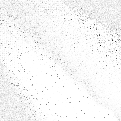
\includegraphics[width=\textwidth]{images/findings/experiments/regularization/strats/0.60/crib_min_avg.png}
		\caption{\cribminavg}
	\end{subfigure}
	~
	\begin{subfigure}[t]{0.22\textwidth}
		\center
		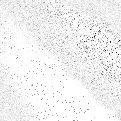
\includegraphics[width=\textwidth]{images/findings/experiments/regularization/strats/0.60/pegging_max_avg_gained.png}
		\caption{\peggingmaxavggained}
	\end{subfigure}
~
	\begin{subfigure}[t]{0.22\textwidth}
		\center
		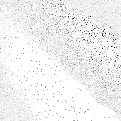
\includegraphics[width=\textwidth]{images/findings/experiments/regularization/strats/0.60/pegging_max_med_gained.png}
		\caption{\peggingmaxmedgained}
	\end{subfigure}
	~
	\begin{subfigure}[t]{0.22\textwidth}
		\center
		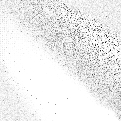
\includegraphics[width=\textwidth]{images/findings/experiments/regularization/strats/0.60/pegging_min_avg_given.png}
		\caption{\peggingminavggiven}
	\end{subfigure}

\caption{
	Final strategies for an agent using regularized learning
	when playing as the dealer
	and the maximum value weight allowed is 0.60
	after training for 500,000 games.
}
\label{fig:neighbor-strats}
\end{figure}


\begin{figure}
\center

	\begin{subfigure}[t]{0.22\textwidth}
		\center
		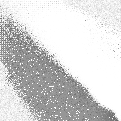
\includegraphics[width=\textwidth]{images/findings/experiments/regularization/strats/0.70/hand_max_min.png}
		\caption{\handmaxmin}
	\end{subfigure}
	~
	\begin{subfigure}[t]{0.22\textwidth}
		\center
		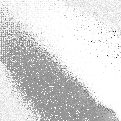
\includegraphics[width=\textwidth]{images/findings/experiments/regularization/strats/0.70/hand_max_avg.png}
		\caption{\handmaxavg}
	\end{subfigure}
~
	\begin{subfigure}[t]{0.22\textwidth}
		\center
		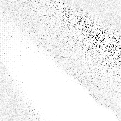
\includegraphics[width=\textwidth]{images/findings/experiments/regularization/strats/0.70/hand_max_med.png}
		\caption{\handmaxmed}
	\end{subfigure}
	~
	\begin{subfigure}[t]{0.22\textwidth}
		\center
		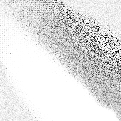
\includegraphics[width=\textwidth]{images/findings/experiments/regularization/strats/0.70/hand_max_poss.png}
		\caption{\handmaxposs}
	\end{subfigure}

	\begin{subfigure}[t]{0.22\textwidth}
		\center
		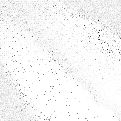
\includegraphics[width=\textwidth]{images/findings/experiments/regularization/strats/0.70/crib_min_avg.png}
		\caption{\cribminavg}
	\end{subfigure}
	~
	\begin{subfigure}[t]{0.22\textwidth}
		\center
		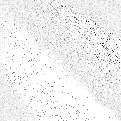
\includegraphics[width=\textwidth]{images/findings/experiments/regularization/strats/0.70/pegging_max_avg_gained.png}
		\caption{\peggingmaxavggained}
	\end{subfigure}
~
	\begin{subfigure}[t]{0.22\textwidth}
		\center
		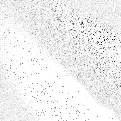
\includegraphics[width=\textwidth]{images/findings/experiments/regularization/strats/0.70/pegging_max_med_gained.png}
		\caption{\peggingmaxmedgained}
	\end{subfigure}
	~
	\begin{subfigure}[t]{0.22\textwidth}
		\center
		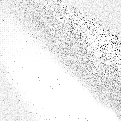
\includegraphics[width=\textwidth]{images/findings/experiments/regularization/strats/0.70/pegging_min_avg_given.png}
		\caption{\peggingminavggiven}
	\end{subfigure}

\caption{
	Final strategies for an agent using regularized learning
	when playing as the pone
	and the maximum value weight allowed is 0.70
	after training for 500,000 games.
}
\label{fig:reg-strats-0.70}
\end{figure}


\begin{figure}
\center

	\begin{subfigure}[t]{0.22\textwidth}
		\center
		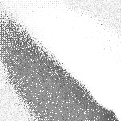
\includegraphics[width=\textwidth]{images/findings/experiments/regularization/strats/0.80/hand_max_min.png}
		\caption{\handmaxmin}
	\end{subfigure}
	~
	\begin{subfigure}[t]{0.22\textwidth}
		\center
		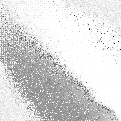
\includegraphics[width=\textwidth]{images/findings/experiments/regularization/strats/0.80/hand_max_avg.png}
		\caption{\handmaxavg}
	\end{subfigure}
~
	\begin{subfigure}[t]{0.22\textwidth}
		\center
		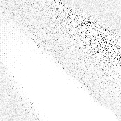
\includegraphics[width=\textwidth]{images/findings/experiments/regularization/strats/0.80/hand_max_med.png}
		\caption{\handmaxmed}
	\end{subfigure}
	~
	\begin{subfigure}[t]{0.22\textwidth}
		\center
		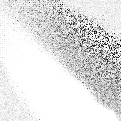
\includegraphics[width=\textwidth]{images/findings/experiments/regularization/strats/0.80/hand_max_poss.png}
		\caption{\handmaxposs}
	\end{subfigure}

	\begin{subfigure}[t]{0.22\textwidth}
		\center
		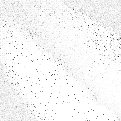
\includegraphics[width=\textwidth]{images/findings/experiments/regularization/strats/0.80/crib_min_avg.png}
		\caption{\cribminavg}
	\end{subfigure}
	~
	\begin{subfigure}[t]{0.22\textwidth}
		\center
		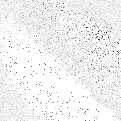
\includegraphics[width=\textwidth]{images/findings/experiments/regularization/strats/0.80/pegging_max_avg_gained.png}
		\caption{\peggingmaxavggained}
	\end{subfigure}
~
	\begin{subfigure}[t]{0.22\textwidth}
		\center
		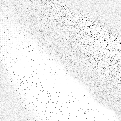
\includegraphics[width=\textwidth]{images/findings/experiments/regularization/strats/0.80/pegging_max_med_gained.png}
		\caption{\peggingmaxmedgained}
	\end{subfigure}
	~
	\begin{subfigure}[t]{0.22\textwidth}
		\center
		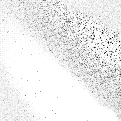
\includegraphics[width=\textwidth]{images/findings/experiments/regularization/strats/0.80/pegging_min_avg_given.png}
		\caption{\peggingminavggiven}
	\end{subfigure}

\caption{
	Final strategies for an agent using regularized learning
	when playing as the dealer
	and the maximum value weight allowed is 0.80
	after training for 500,000 games.
}
\label{fig:reg-strats-0.80}
\end{figure}


%%%
As expected,
the limitation of maximum attainable value did indeed force the agent to learn
multiple applicable strategies for each score location.
%
As can be seen in Figure~\ref{fig:r2-reg},
the \handmaxmin\ and \handmaxavg\ strategies are now equally represented across
the winning triangle area.
%
This is demonstrated by the monotone gray seen in these locations.
%
Rather than each strategy specializing to its own dominant location,
the territory is shared between the two most most applicable strategies.
%
Therefore,
the regularization does indeed prevent the dominance of a single strategy
unintentionally discarding all other potential strategies.
%%%

%%%
Additionally understandably,
the nature of this gray mass alters significantly as the regularization rate is
altered.
%
With a lower allowed maximum value,
the strategy graphs take on the previously mentioned slightly amorphous gray
blob shape.
%
As the maximum value approaches one,
the gray shape begins to specialize more and begins to show resemblance to the
final strategy graphs obtained without regularization.
%%%

%%%%
%Interestingly,
%even with this regularization,
%small \textit{islands} of
%\cribminavg, \peggingmaxavggained, and \peggingminavggiven
%are seen to still exist in the \handmaxmin/\handmaxavg-dominated territory.
%%
%This indicates that regularization is not capable of addressing the situations
%in which single score locations may benefit from
%%%%

